\documentclass{article}

\usepackage[T1]{fontenc}

\usepackage{polski}
\usepackage[utf8]{inputenc}
\usepackage[polish]{babel}
\let\lll\undefined
\usepackage{amssymb}
\usepackage{amsmath}
\usepackage{algorithm}
\usepackage{algpseudocode}
\usepackage{graphicx}
\usepackage{floatpag}



\title{Pracownia z analizy numerycznej \\ Sprawozdanie do zadania P1.16}
\author{Mikołaj Słupiński}
\date{Wrocław, dnia 30 października 2016 r.}

\begin{document}
  \maketitle
  \section{Wstęp}
    \paragraph{} Obliczanie miejsc zerowych układów równań jest zadaniem nie tylko
    interesującym, ale również niezwykle potrzebnym w problemach inżynierskich.

    Niejednokrotnie chcielibyśmy nie tylko poznać rozwiązanie układu równań, ale
    zrobić to w sposób efektywny. Przez lata opracowano wiele metod rozwiązywania
    układów równań nieliniowych.

    Wśród wielu dostępnych metod szczególne zainteresowanie wzbudza metoda Newtona.

    Głównym celem niniejszego sprawozdania jest omówienie użycia metody Newtona
    do rozwiązania układów równań liniowych oraz analiza działania samego algorytmu

  \section{Działanie metody Newtona dla układu równań nieliniowych}

    \paragraph{} Metoda Newtona rozwiązywania układu równań nieliniowych jest pewnym
    uogólnieniem standardowej metody Newtona rozwiązywania pojedynczego równania nieliniowego.

    Zapiszmy układ równań nieliniowych,
    \begin{equation*}
      f_{i}(x_{1}, x_{2},...,x_{n}) = 0 \quad(i = 1, 2, ..., n),
    \end{equation*}
    w postaci wektorowej,
    \begin{equation*}
      f(x) = 0,
    \end{equation*}
    gdzie $f, x \in \mathbb{R}^n$. Dla wektora $x_{k}$ będącego bieżącym przybliżeniem
    rozwiązania układu, kolejne przybliżenie $x_{k+1}$ jest rozwiązaniem następującego
    układu równań liniowych:


    \begin{equation}\label{eq:rownanie1}
      J(x_{k})(x_{k+1} - x_{k}) = -f(x_{k})
    \end{equation}

    gdzie
    \begin{equation*}
      J(x) =
      \begin{pmatrix}
        \frac{\partial f_{1}}{\partial x_{1}} & \cdots & \frac{\partial f_{1}}{\partial x_{n}} \\
        \vdots & \ddots & \vdots \\
        \frac{\partial f_{n}}{\partial x_{1}} & \cdots & \frac{\partial f_{n}}{\partial x_{n}}
      \end{pmatrix} \in \mathbb{R}^{n \times n}.
    \end{equation*}

    Zauważmy, że równanie \eqref{eq:rownanie1} możemy przekształcić do postaci:

    \begin{equation}\label{eq:rownanie2}
      x_{k+1} = x_{k} - J^{-1}\cdot f(x_{k}).
    \end{equation}

    Łatwo w tym miejscu zauważyć analogię do równania
    \begin{equation*}
      x_{k+1} = x_{k} - \frac{f(x_{k})}{f'(x_{k})}
    \end{equation*}
    używanego w metodzie Newtona dla pojedynczego równania nieliniowego.

    Wielowymiarowość funkcji $f(x_{n})$ wymusza zastanowienie się jak powinno wyglądać
    jej kryterium zbieżności.
    Możemy uznać, że wartości funkcji $f(x_{n})$ śa dostatecznie blisko miejsca
    zerowego, gdy maksimum z wartości bezwzględnych funkcji $f_{i}(x_{n})$ jest
    mniejsza niż pewna ustalona wartość $\varepsilon > 0$, tzn.

    \begin{equation*}
      max_{i}|f_{i}(x_{n})| < \varepsilon.
    \end{equation*}

    Inną możliwością jest sprawdzenie, czy norma wektora $f(x_{n})$ jest mniejsza
    od ustalonej wartości, tzn.
    \begin{equation*}
      \lVert f(x_{n})\rVert < \varepsilon.
    \end{equation*}

  \section{Problemy}
    \paragraph{} Należy mieć świadomość, że metoda Newtona nie jest pozbawiona wad
    i może sprawiać pewne problemy.

    Na samym początku należy zauważyć, że aby rozwiązać układ równań musimy być w stanie
    policzyć wszystkie pochodne cząstkowe funkcji składowych $f_i(x)$ funkcji $f(x)$. Co więcej
    funkcje te muszą być różniczkowalne.

    Wróćmy do wzoru \eqref{eq:rownanie2}. Zauważmy, że używamy w nim macierzy odwrotnej
    do macierzy $J$. Musimy mieć świadomość, że nie każda macierz jest odwracalna.
    Co więcej sama operacja odwracania macierzy jest dosyć kosztowna, co zwiększa
    nam czas działania programu.

    Należy zauważyć, że metoda Newtona dla układu równań, podobnie jak
    metoda Newtona dla pojedynczego równania jest zbieżna jedynie lokalnie, więc
    w przypadku złego doboru miejsca startowego $x_0$ może ona zbiegać zbyt długo
    lub być rozbieżna.

    W tym momencie trzeba zastanowić się, jak efektywnie znaleźć miejsce startowe
    dla metody Newtona. O ile w przypadku pojedynczego równania możemy posiłkować
    się twierdzeniem o wartości średniej, o tyle uogólnienie wielowymiarowe już
    na to nie pozwala. Zawsze warto posługiwać się informacjami o samym problemie
    inżynierskim, który próbujemy rozwiązać. Natomiast, jeżeli jesteśmy pozbawieni
    jakichkolwiek informacji o problemie, z którym związany jest dany układ równań,
    możemy spróbować podejścia randomizowanego, tzn. wylosować kilka punktów startowych
    i badać zbieżność na nich.

  \section{Algorytm wyszukiwania rozwiązania}
    \paragraph{} Mając powyższe informacje możemy stworzyć algorytm znajdowania miejsc zerowych

    \begin{algorithm}
    \caption{Algorytm Newtona}\label{alg:newton}
      \begin{algorithmic}[1]
      \Procedure{Newton}{$x_0, f, J, maxIter, \varepsilon, maxVal$}
        \State $x_n\gets x_0$
        \State $N\gets maxIter$
        \While{$N>0$}
          \If{$det(J(x_n))=0$}
            \State \Return $-2$
          \EndIf
          \State $J_{x}\gets J^{-1}(x_n)$
          \State $x_n\gets x_n-J_{x}\cdot f(x_n)$
          \If{$\lVert f(x_n)\rVert < \varepsilon$}
            \State \Return $0$
          \EndIf
          \If{$\lVert f(x_n)\rVert > maxVal$}
            \State \Return $-3$
          \EndIf
          \State $N \gets N - 1$
        \EndWhile
        \State \Return $-1$
        \EndProcedure
      \end{algorithmic}
    \end{algorithm}

    W powyższym algorytmie założono, że jesteśmy w stanie efektywnie obliczyć odwrotność
    macierzy $J$ w punkcie $x_n$. W swojej implementacji powyższego algorytmu
    użyłem odwracania macierzy metodą rozkładu LU.
  \section{Szacowanie złożoności obliczeniowej metody Newtona}
    \paragraph{} Dla funkcji $f(x)$ gdzie $f, x \in \mathbb{R}^n$ możemy uzależnić
    czas działania algorytmu od wielkości $n$.

    Na samym początku nasz algorytm oblicza wartość jakobianu funkcji $f$. Aby
    tego dokonoć musi dokonać ewaluacji $n^2$ funkcji.

    Następnie potrzebujemy obliczyć wartość wyznacznika Jakobianu. Jeżeli przyjmiemy,
    że w implementacji użyto metody rozkładu LU, możemy sprawdzić, czy macierz
    jest odwracalna w trakcie rozkładu na macierz górno oraz dolnotrójkątną.

    Najbardziej czasochłonną operacją jest proces odwracania macierzy. Klasyczna
    eliminacja Gaussa daje nam złożoność obliczeniową rzędu $O(n^4)$\cite{vanderberghe}, natomiast
    zastosowana w dołączonym do sprawozdania programie \texttt{program.jl} metoda
    rozkładu LU ma złożoność rzędu $O(n^3) \cite{vanderberghe}$.

    Aby obliczyć wartość $x_n$ potrzebujemy najpierw obliczyć wartość wyrażenia
    $x_n-J_{x}\cdot f(x_n)$. Zauważmy, że aby obliczyć iloczyn skalarny dwóch
    wektorów potrzebujemy wykonać $n$ mnożeń oraz $n-1$ dodawań. A zatem złożoność obliczania
    iloczynu skalarnego wynosi $n(n-1)$. Następnie zauważmy, że mnożenie macierzy
    przez wektor, to iloczyn skalarny wierszy macierzy i wektora. Mamy n wierszy, czyli
    złożoność obliczania iloczynu $x_n-J_{x}\cdot f(x_n)$ to $n^2(n-1)$.

    Następnie odejmujemy od $x_n$ wartość obliczonego iloczynu, czyli wykonujemy
    $n$ odejmowań.

    Następnie dwukrotnie sprawdzamy normę wektora o długości $n$. Obliczanie normy
    to kolejny przypadek obliczania iloczyny skalarnego, a zatem znowu wykonujemy
    $n(n-1)$ operacji.

    W rezultacie otrzymujemy złożoność $n^2 + O(n^3) + n^2(n-1) + n + 2n(n-1) = n^3 +2n^2 - n + O(n^3) = O(n^3)$
    dla pojedynczej iteracji.

  \section{Przykłady obliczania układów równań dwóch zmiennych}
    \paragraph{} Spróbujemy rozwiązać kilka układów równań za pomocą zaimplementowanej
    przeze mnie metody Newtona. W poniższych przykładach $f, g, X \in \mathbb{R}^2$ oraz
    $X = \begin{pmatrix} x \\ y \end{pmatrix}$.

    Obliczenia wykonano za pomocą załączonego programu \texttt{program.jl}.
    W obu przykładach wykonano je z dokładnością $\varepsilon = 10^{-14}$

    Na samym początku rozważmy układ równań
    \begin{equation}\label{eq.fx}
      \begin{cases}
        x + e^{-x} + y^3        &= 0 \\
        x^2 + 2xy - y^2 + tan x &= 0
      \end{cases}
    \end{equation}
    Niech $f(X) = 0$ bedzie funkcją zadaną przez układ równań \eqref{eq.fx}.
    Wtedy Jakobian oznaczamy przez $J_f$ i
    \begin{equation*}
      J_{f}(X) =
      \begin{pmatrix}
        1 - e^{-x}              & 3y^2    \\
        2x + 2y + 1 + (tan x)^2 & 2x - 2y
      \end{pmatrix}
    \end{equation*}

    W tabeli nr \ref{tab:f} pokazano wyniki kolejnych iteracji programu. Jak widać,
    metoda Newtona okazała się w tym przypadku zbieżna już dla 10 iteracji.

    Na wykresie nr \ref{fig:plot1} pokazano jak wyglądała wartość normy z $f(X_n)$
    dla poszczególnych wartości zmiennej $X_n$.

    \begin{table}[htb]
      \centering
      \caption{Wartości kolejnych przybliżeń $X_n$ dla funkcji $f$}
      \label{tab:f}
      \begin{tabular}{|c|c|c|c|}
        \hline
        n  & $X_n$                                                         & $f(X_n)$                                                                                  & $\lVert f(X_n)\rVert$          \\ \hline
        0  & $\begin{pmatrix} 3.1          \\ 1.5           \end{pmatrix}$ & $\begin{pmatrix} 6.5200492024                \\ 16.6183833454              \end{pmatrix}$ & $ 17.8516583716 $              \\ \hline
        1  & $\begin{pmatrix} 1.7124344144 \\ 0.7303715052  \end{pmatrix}$ & $\begin{pmatrix} 2.2824716679                \\ -2.1125561781              \end{pmatrix}$ & $ 3.1100756455 $               \\ \hline
        2  & $\begin{pmatrix} 1.8033289693 \\ -0.7424309818 \end{pmatrix}$ & $\begin{pmatrix} 1.5588477469                \\ -4.1995827405              \end{pmatrix}$ & $ 4.4795648775 $               \\ \hline
        3  & $\begin{pmatrix} 2.2929266067 \\ -1.9324231030 \end{pmatrix}$ & $\begin{pmatrix} -4.8222713258               \\ -8.4738301857              \end{pmatrix}$ & $ 9.7498768579 $               \\ \hline
        4  & $\begin{pmatrix} 4.3670510738 \\ -1.6684196099 \end{pmatrix}$ & $\begin{pmatrix} -0.2645131821               \\ 4.4950399716               \end{pmatrix}$ & $ 4.5028159601 $               \\ \hline
        5  & $\begin{pmatrix} 3.9829061047 \\ -1.5913277937 \end{pmatrix}$ & $\begin{pmatrix} -0.0282202771               \\ 1.7735834199               \end{pmatrix}$ & $ 1.7738079184 $               \\ \hline
        6  & $\begin{pmatrix} 3.6584660162 \\ -1.5457023040 \end{pmatrix}$ & $\begin{pmatrix} -0.0087471308               \\ 0.2537968804               \end{pmatrix}$ & $ 0.2539475709 $               \\ \hline
        7  & $\begin{pmatrix} 3.5939994766 \\ -1.5357195526 \end{pmatrix}$ & $\begin{pmatrix} -0.0004063946               \\ 0.0056741198               \end{pmatrix}$ & $ 0.0056886547 $               \\ \hline
        8  & $\begin{pmatrix} 3.5924108303 \\ -1.5354437522 \end{pmatrix}$ & $\begin{pmatrix} -3.1572096226\cdot 10^{-7}  \\ 3.0850043851\cdot 10^{-6}  \end{pmatrix}$ & $ 3.1011178278\cdot 10^{-6}$   \\ \hline
        9  & $\begin{pmatrix} 3.5924099307 \\ -1.5354435838 \end{pmatrix}$ & $\begin{pmatrix} -1.1945999745\cdot 10^{-13} \\ 9.6073149436\cdot 10^{-13} \end{pmatrix}$ & $ 9.6812999915\cdot 10^{-13} $ \\ \hline
        10 & $\begin{pmatrix} 3.5924099307 \\ -1.5354435838 \end{pmatrix}$ & $\begin{pmatrix} 0.0                         \\ 6.6613381478\cdot 10^{-16} \end{pmatrix}$ & $ 6.6613381478\cdot 10^{-16} $ \\ \hline
      \end{tabular}
    \end{table}
    \begin{figure}
      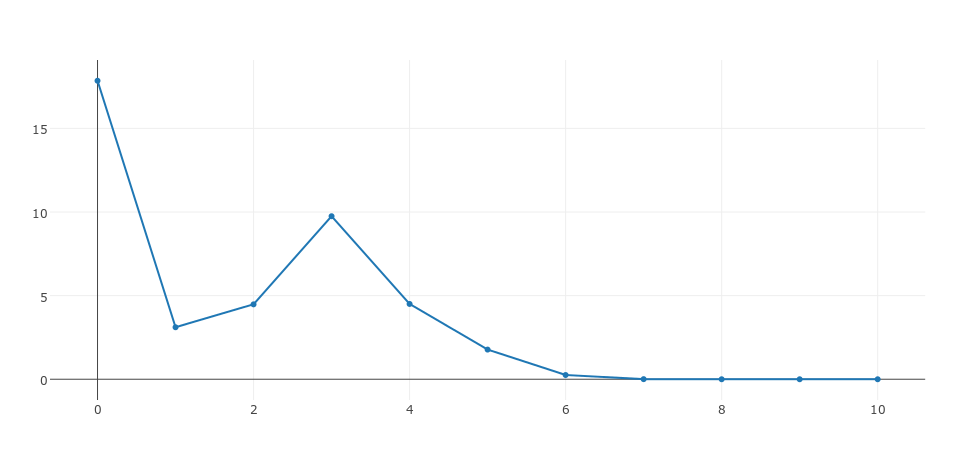
\includegraphics[width=\linewidth]{fplot.png}
      \caption{Wykres normy funkcji $f(X_n)$}
      \label{fig:plot1}
    \end{figure}

    Weźmy teraz układ równań
    \begin{equation}\label{eq.gx}
      \begin{cases}
        x^3 + y - 1 &= 0 \\
        y^3 - x + 1 &= 0 \\
      \end{cases}
    \end{equation}
    Niech $g(X) = 0$ bedzie funkcją zadaną przez układ równań \eqref{eq.gx}.
    Wtedy Jakobian tej oznaczamy przez $J_g$ i
    \begin{equation*}
      J_{g}(X) =
      \begin{pmatrix}
        3x^2 & 1    \\
        -1   & 3y^2
      \end{pmatrix}
    \end{equation*}

    W tabeli nr \ref{tab:g} pokazano wyniki kolejnych iteracji programu. W tym przypadku
    metoda Newtona ma podobną wydajność co dla funkcji $f $. Program
    znalazł odpowiednie przybliżenie miejsca zerowego już po 9 iteracjach.

    Na wykresie nr \ref{fig:plot2} pokazano jak wyglądała wartość normy z $g(X_n)$
    dla poszczególnych iteracji wartości zmiennej $X_n$.



    \begin{table}[htb]
      \centering
      \caption{Wartości kolejnych przybliżeń $X_n$ dla funkcji $g$}
      \label{tab:g}
      \begin{tabular}{|c|c|c|c|}
        \hline
        n & $X_n$                                                                       & $g(X_n)$                                                                                   & $\lVert g(X_n)\rVert$           \\ \hline
        0 & $\begin{pmatrix} 4.0          \\ 1.0                         \end{pmatrix}$ & $\begin{pmatrix} 64.0                        \\ -2.0                        \end{pmatrix}$ & $ 64.0312423743 $               \\ \hline
        1 & $\begin{pmatrix} 2.6620689655 \\ 1.2206896552                \end{pmatrix}$ & $\begin{pmatrix} 19.0857373406               \\ 0.1568602239                \end{pmatrix}$ & $ 19.0863819244 $               \\ \hline
        2 & $\begin{pmatrix} 1.7753132333 \\ 0.9872315655                \end{pmatrix}$ & $\begin{pmatrix} 5.5825521046                \\ 0.1868684802                \end{pmatrix}$ & $ 5.5856788154 $                \\ \hline
        3 & $\begin{pmatrix} 1.2120269729 \\ 0.7306700350                \end{pmatrix}$ & $\begin{pmatrix} 1.5111490306                \\ 0.1780621956                \end{pmatrix}$ & $ 1.5216036074 $                \\ \hline
        4 & $\begin{pmatrix} 0.9337790284 \\ 0.4457675281                \end{pmatrix}$ & $\begin{pmatrix} 0.2599698712                \\ 0.1547988528                \end{pmatrix}$ & $ 0.3025673789 $                \\ \hline
        5 & $\begin{pmatrix} 0.9337102753 \\ 0.1859775033                \end{pmatrix}$ & $\begin{pmatrix} 1.3241557406 \cdot 10^{-8}  \\ 0.0727222461                \end{pmatrix}$ & $ 0.0727222461 $                \\ \hline
        6 & $\begin{pmatrix} 0.9909094568 \\ 0.0363761977                \end{pmatrix}$ & $\begin{pmatrix} 0.0093517308                \\ 0.0091386772                \end{pmatrix}$ & $ 0.0130755608 $                \\ \hline
        7 & $\begin{pmatrix} 0.9999058116 \\ 0.0005238627                \end{pmatrix}$ & $\begin{pmatrix} 0.0002413241                \\ 9.4188563688 \cdot 10^{-5}  \end{pmatrix}$ & $ 0.0002590537 $                \\ \hline
        8 & $\begin{pmatrix} 0.9999999997 \\ 2.7475062468 \cdot 10^{-8}  \end{pmatrix}$ & $\begin{pmatrix} 2.6612541504 \cdot 10^{-8}  \\ 2.8750701819 \cdot 10^{-10} \end{pmatrix}$ & $ 2.6614094491 \cdot 10^{-8} $  \\ \hline
        9 & $\begin{pmatrix} 1.0          \\ -9.035999581 \cdot 10^{-17} \end{pmatrix}$ & $\begin{pmatrix} -1.110223025 \cdot 10^{-16} \\ 0.0                         \end{pmatrix}$ & $ 1.1102230246 \cdot 10^{-16} $ \\ \hline
      \end{tabular}
    \end{table}
    \begin{figure}
      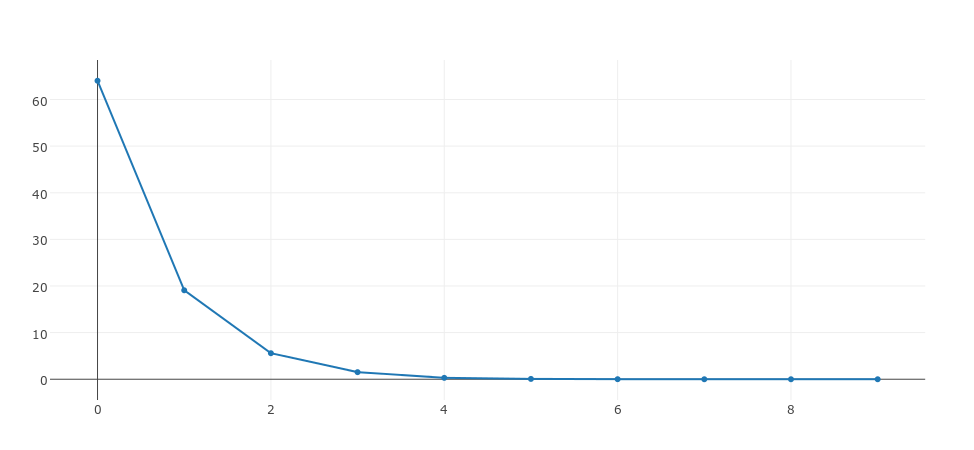
\includegraphics[width=\linewidth]{gplot.png}
      \caption{Wykres normy funkcji $g(X_n)$}
      \label{fig:plot2}
    \end{figure}

    Jak widać, algorytm okazał się wydajny dla zadanych równań. Potrzebował niewielu
    iteracji, żeby znaleźć odpowiednie przybliżenia dla miejsc zerowych funkcji
    $f$ i $g$.

  \section{Rozwiązanie układu równań trzech zmiennych}
    \paragraph{} Aby nie ograniczać się tylko do układów z dwoma zmiennymi przetestowano program
    dla ukladu równań trzech zmiennych.

    Niech
    \begin{equation}\label{eq.hx}
      \begin{cases}
        xy - x^2 - 1        &= 0 \\
        xyz + y^2 - x^2 - 2 &= 0 \\
        e^x + z - e^y - 3   &= 0
      \end{cases}
    \end{equation}
    Niech $h(X) = 0$ bedzie funkcją zadaną przez układ równań \eqref{eq.hx}.
    Wtedy Jakobian oznaczamy przez $J_h$ i
    \begin{equation*}
      J_{h}(X) =
      \begin{pmatrix}
        y     & z       & -2z \\
        yz-2x & xz + 2y & xy  \\
        e^x   & e^y     & 1
      \end{pmatrix}
    \end{equation*}

    Wywołanie programu dla układu równań \eqref{eq.hx} z dokładnością $\varepsilon = 10^{-10}$
    wymagało 91 iteracji programu. W tabeli nr \ref{tab:h} pokazano wyniki dla wartości
    początkowej $X_0$ oraz 14 oszacowań zmiennej $X_n$.

    \begin{table}[htb]
      \thisfloatpagestyle{empty}
      \centering
      \caption{Wartości kolejnych przybliżeń $X_n$ dla funkcji $h$}
      \label{tab:h}
      \begin{tabular}{|c|c|c|c|}
        \hline
        n      & $X_n$                                                                              & $h(X_n)$                                                                                                               & $ \lVert h(X_n)\rVert$        \\ \hline
        0      & $\begin{pmatrix} 1.0            \\ 1.0            \\ 1.0            \end{pmatrix}$ & $\begin{pmatrix} -1.0                       \\ -1.0                       \\ -2.0                       \end{pmatrix}$ & $ 2.4494897428 $              \\ \hline
        1      & $\begin{pmatrix} 1.1789564011   \\ 0.9414877273   \\ 2.3544932192   \end{pmatrix}$ & $\begin{pmatrix} -5.4336653368              \\ 0.1098848060               \\ 0.0416801252               \end{pmatrix}$ & $ 5.4349361446 $              \\ \hline
        2      & $\begin{pmatrix} 1.7215915984   \\ 1.2041400775   \\ 1.2221032822   \end{pmatrix}$ & $\begin{pmatrix} -0.4204989917              \\ -0.9804584447              \\ 0.4816361928               \end{pmatrix}$ & $ 1.1705091140 $              \\ \hline
        3      & $\begin{pmatrix} 1.4458386353   \\ 1.0498771911   \\ 1.7685746528   \end{pmatrix}$ & $\begin{pmatrix} -2.6099032973              \\ -0.3035940339              \\ 0.1566854600               \end{pmatrix}$ & $ 2.6321692369 $              \\ \hline
        4      & $\begin{pmatrix} 1.7476807102   \\ 1.3610798462   \\ 1.2196449344   \end{pmatrix}$ & $\begin{pmatrix} -0.1088007738              \\ -0.3006398725              \\ 0.0605136204               \end{pmatrix}$ & $ 0.3253979711 $              \\ \hline
        \vdots & \vdots                                                                             & \vdots                                                                                                                 & \vdots                        \\ \hline
        40     & $\begin{pmatrix} 1.7776824568   \\ 1.4239719540   \\ 1.2374559377   \end{pmatrix}$ & $\begin{pmatrix} 7.2763831434\cdot 10^{5}   \\ -1.9603114687\cdot 10^{9}  \\ 3.2317526433\cdot 10^{10}  \end{pmatrix}$ & $ 7.2763831461\cdot 10^{5}$   \\ \hline
        41     & $\begin{pmatrix} 1.7776638528   \\ 1.4239519070   \\ 1.2374827343   \end{pmatrix}$ & $\begin{pmatrix} -5.5684352006\cdot 10^{5}  \\ -1.1475393968\cdot 10^{9}  \\ 1.8918910882\cdot 10^{10}  \end{pmatrix}$ & $ 5.5684352018\cdot 10^{5}$   \\ \hline
        42     & $\begin{pmatrix} 1.7776780881   \\ 1.4239672465   \\ 1.2374622305   \end{pmatrix}$ & $\begin{pmatrix} 4.2600372742\cdot 10^{5}   \\ -6.7185546015\cdot 10^{10} \\ 1.1076206619\cdot 10^{10}  \end{pmatrix}$ & $ 4.2600372747\cdot 10^{5}$   \\ \hline
        43     & $\begin{pmatrix} 1.7776671965   \\ 1.4239555102   \\ 1.2374779183   \end{pmatrix}$ & $\begin{pmatrix} -3.2598584530\cdot 10^{5}  \\ -3.9330894097\cdot 10^{10} \\ 6.4843241887\cdot 10^{11}  \end{pmatrix}$ & $ 3.2598584533\cdot 10^{5}$   \\ \hline
        44     & $\begin{pmatrix} 1.7776755303   \\ 1.4239644903   \\ 1.2374659147   \end{pmatrix}$ & $\begin{pmatrix} 2.4940414007\cdot 10^{5}   \\ -2.3026602847\cdot 10^{10} \\ 3.7960745658\cdot 10^{11}  \end{pmatrix}$ & $ 2.4940414008\cdot 10^{5}$   \\ \hline
        \vdots & \vdots                                                                             & \vdots                                                                                                                 & \vdots                        \\ \hline
        87     & $\begin{pmatrix} 1.777671918075 \\ 1.423960597849 \\ 1.237471117784 \end{pmatrix}$ & $\begin{pmatrix} -2.4987945046\cdot 10^{10} \\ 1.3322676296\cdot 10^{15}  \\ 0.0                        \end{pmatrix}$ & $ 2.4987945047\cdot 10^{10} $ \\ \hline
        88     & $\begin{pmatrix} 1.777671918038 \\ 1.423960597918 \\ 1.237471117692 \end{pmatrix}$ & $\begin{pmatrix} 1.9119705819\cdot 10^{10}  \\ -4.4408920985\cdot 10^{16} \\ -8.8817841970\cdot 10^{16} \end{pmatrix}$ & $ 1.9119705819\cdot 10^{10} $ \\ \hline
        89     & $\begin{pmatrix} 1.777671917990 \\ 1.423960597866 \\ 1.237471117762 \end{pmatrix}$ & $\begin{pmatrix} -1.4629542022\cdot 10^{10} \\ -4.4408920985\cdot 10^{16} \\ 8.8817841970\cdot 10^{16}  \end{pmatrix}$ & $ 1.4629542023\cdot 10^{10} $ \\ \hline
        90     & $\begin{pmatrix} 1.777671918027 \\ 1.423960597906 \\ 1.237471117708 \end{pmatrix}$ & $\begin{pmatrix} 1.1193557192\cdot 10^{10}  \\ 8.8817841970\cdot 10^{16}  \\ 0.0                        \end{pmatrix}$ & $ 1.1193557193\cdot 10^{10} $ \\ \hline
        91     & $\begin{pmatrix} 1.777671917998 \\ 1.423960597875 \\ 1.237471117750 \end{pmatrix}$ & $\begin{pmatrix} -8.5642382075\cdot 10^{11} \\ -1.3322676296\cdot 10^{15} \\ 0.0                        \end{pmatrix}$ & $ 8.5642382085\cdot 10^{11} $ \\ \hline
      \end{tabular}
    \end{table}

    Jak widać z danych zawartych w tabeli nr \ref{tab:h} oraz wykresu nr \ref{fig:plot3},
    dla początkowych wartość $X_n$ występują duże wahania wartości normy funkcji
    $h$, które w pewnym momencie się stabilizują aż norma zaczyna być ściśle malejąca
    maleć.

    Na przykładzie tym widać, że metoda Newtona dla funkcji wielu zmiennych może
    być mało efektywna.
    \begin{figure}
      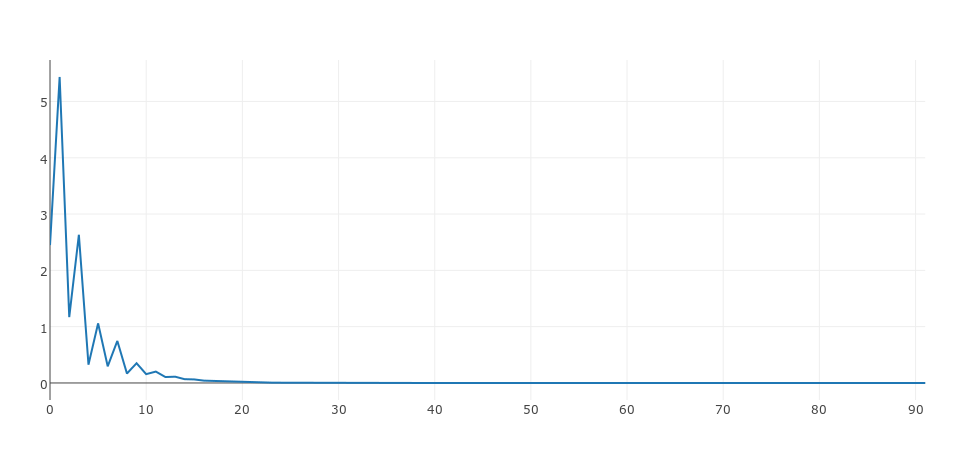
\includegraphics[width=\linewidth]{hplot.png}
      \caption{Wykres normy funkcji $h(X_n)$}
      \label{fig:plot3}
    \end{figure}
  \section{Wnioski}
    \paragraph{} Metoda Newtona rozwiązywania układów równać, choć niewątpliwie
    użyteczna, nie jest pozbawiona wad. Wymaga ona znajomości pochodnych cząstkowych
    funkcji, które chcemy obliczyć, co o ile nie sprawia większych problemów w
    przypadku niewielkiej liczby zmiennych, o tyle dla dużej ich ilości może być
    zadaniem problematycznym.

    Kluczowym elementem metody Newtona jest obliczenie macierzy odwrotnej, co jest
    zadaniem o dużej złożoności obliczeniowej.

    Jak pokazano na przykładzie funkcji trzech zmiennych, funkcja może wykonać bardzo
    dużo iteracj, zanim pozyskamy pożądaną dokładność.

    Nie można jednak stwierdzić, że metoda ta jest zła, gdyż dla prostych układów
    pozwala nam ona uzyskać satysfakcjonujący wynik w niewielkiej liczbie iteracji
    i jest ona prosta w implementacji.


    \begin{thebibliography}{9}
      \bibitem{kincaid}
        David Kincaid, Ward Cheney.
        \textit{Analiza Numeryczna}.
        Wydawnictwa Naukowo-Techniczne, Warszawa, 2006.

      \bibitem{bjorck}
        Ake Bjorck, Germund Dahlquist.
        \textit{Metody numeryczne}.
        Państwowe Wydawnictwo Naukowe, 1987.

      \bibitem{vanderberghe}
        Lieven Vandenberghe:  LU factorization,\\
        \texttt{https://www.seas.ucla.edu/\~{}vandenbe/103/lectures/lu.pdf}
    \end{thebibliography}


\end{document}
